


\section*{Learning Objectives}
\begin{itemize}
\item Provide motivation for considering equations with derivatives.
\item Provide a numerical means to approximate a solution to a differential equation.
\item Prepare you a bit for Math 216.
\end{itemize}

\section*{Outcomes}
\begin{itemize}
\item See $F=ma$ in a new light
\item Define an ordinary differential equation, aka an ODE
\item Learn how to pass from a differential equation to a difference equation
\item Relate the process of iterating a difference equation to the process of solving an ODE
\end{itemize}


\vspace*{1.5cm}





\newpage

Equations with a derivative in them are called \textbf{differential equations}. In Robotics, we use differential equations to understand the motion of robots, such as Cassie Blue, or in the case of Project \#3, a Segway. The topic of differential equations is typically delayed until a fourth-semester Calculus course. Moreover, such courses focus almost exclusively on closed-form solutions to differential equations. As you can imagine, we're not a big fan of that. Here, you will see that tools we have developed so far in ROB 101 allow us to develop elementary numerical tools for analyzing the solutions of interesting differential equations.

\section{Preliminaries: Expanding our Concept of an Equation}

Equations in a scalar variable $x \in \real$ probably seem pretty trivial to you by now. Examples we have seen include:
\begin{itemize}
    \item Linear equation: $ax=b$;
    \item Quadratic equation: $ax^2 + bx + c=0$;
     \item Cubic equation: $ax^3 + bx^2 + cx + d=0$; or
    \item Trigonometric equation: $A \cos(x) + B \sin(x) + C=0$.
\end{itemize}

One obvious way to increase the generality of our analysis tools for equations is to include several variables, $x\in \real^n$, $n > 1$, and we've done a bunch of that in ROB 101 as well, where we studied how to find solutions to
\begin{itemize}
    \item System of linear equations: $Ax=b$; and
    \item System of nonlinear equations: $F(x)=0$.
\end{itemize}
In the case of linear systems, we explored map building and linear regression (easy version of Machine Learning) as cool application problems. For nonlinear systems, we looked at the position of a robot gripper in $\real^2$ and sought values for the angles of its joints so that the gripper could be placed in a desired position. \\
\begin{tcolorbox}
Another way to increase the generality of our analysis tools is to expand our concept of equations to include time as a variable! This is a big conceptual step: instead of the values in our equation depending on constants or other powers of our variable $x$, as in the examples we listed above, we will have the value of our variable $x$ at time $t$ depend on $x$ at some other time, say $t-\delta t$, for some $\delta t>0$. 
\end{tcolorbox}

\section{Time in a Digital Computer is Discrete}

To get our heads around functions that depend on time, we'll start with ``time'' as it is treated in a digital computer, namely, time is a sequential variable, such as 
\begin{equation}
    \label{eq:SeqTime}
    k= 1, 2, 3, \ldots. 
\end{equation}
\textbf{Digital} time is similar to our \textit{human} notion of time in that it is strictly increasing, but whereas our human notion of time is continuous (it can be divided into ever smaller increments as long as we ignore the rules of Quantum Mechanics), \textit{digital} time is fundamentally discrete in that it increases by non-zero increments.  \\

Suppose we denote the value of our variable $x$ at time $k$ by $x[k]$, and we define an \textit{equation for $x$ at the next time}, $k+1$, by
\begin{equation}
    \label{eq:DiscreteEquation01}
    x[k+1]=\frac{1}{2}x[k] + 1.
\end{equation}
Equation~\eqref{eq:DiscreteEquation01} says that if we know the value of our variable $x$ at time $k$, we can find the value of $x$ at time $k+1$ by multiplying $x[k]$ by one-half and adding one to it. That seems easy enough. OK, then, what is the value of $x$ at time $k=4$? \\

To compute $x[4]$, we need to know $x[3]$. To compute $x[3]$, we need to know $x[2]$. To compute $x[2]$, we need to know $x[1]$.  If we suppose that time starts at $k=1$, then we cannot go back any further and we realize that somehow $x[1]$ must be given to us!\\

Equation~\eqref{eq:DiscreteEquation01} is called a \textbf{difference equation} and $\mathbf{x[1]}$ is called its \textbf{initial value}. If we are given that $x[1]=4$, we'd then compute that
\begin{align*}
    x[1]&=\frac{1}{2}x[0] + 1 = 3\\
     x[2]&=\frac{1}{2}x[1] + 1 = \frac{7}{2}\\
     x[3]&=\frac{1}{2}x[2] + 1 = \frac{11}{4}\\
     x[4]&=\frac{1}{2}x[3] + 1 = \frac{19}{8}\\
     \vdots~~~&= \hspace*{1cm} \vdots\\
     x[k+1]&= \frac{1}{2}x[k] + 1
\end{align*}

In Fig.~\ref{fig:Proj03Plot01}, we plot the function $x$ for $k=1:20$. We observe that it seems to converge to $2.0$, which is intriguing. In Fig.~\ref{fig:Proj03Plot02}, we have ``cheated'' and made time look quasi-continuous by ``connecting the dots''. The Julia code for generating $x$ and the plots is given in Sec.~\ref{sec:CodeFigs0102}.\\

It would seem that if we could put the ``dots closer together'', the effect in Fig.~\ref{fig:Proj03Plot02} would be even better. Let's try! \\

\begin{figure}
\centering
\begin{minipage}{.4\textwidth}
  \centering
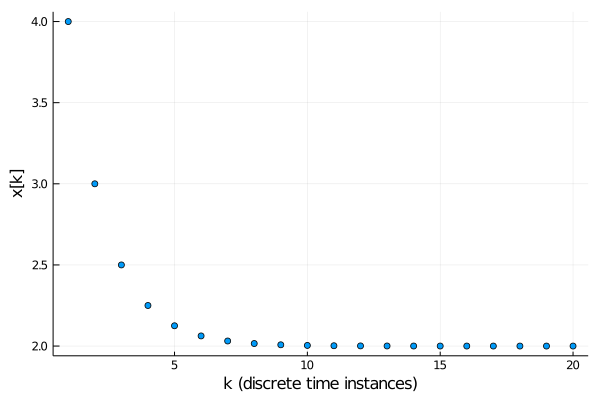
\includegraphics[width=\linewidth]{graphicsAppendices/DiscreteTimeModel.png}
  \caption{Plot of the function $x:[1, 2, \ldots, 20]\to \real$ at discrete instances of time.}
  \label{fig:Proj03Plot01}
\end{minipage}%
\hspace*{1cm}
\begin{minipage}{.4\textwidth}
  \centering
 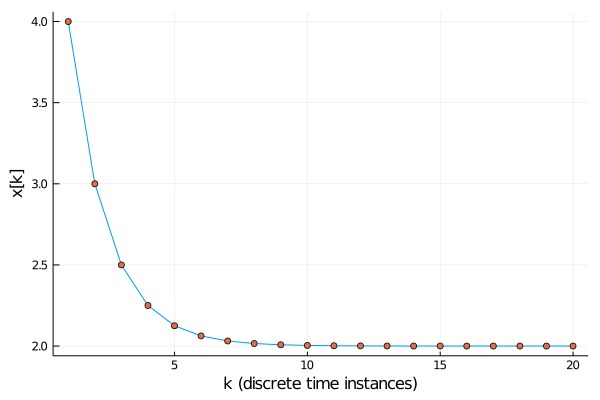
\includegraphics[width=\linewidth]{graphicsAppendices/DiscreteTimeModel02.png}
  \caption{Plot of the function $x:[1, 2, \ldots, 20]\to \real$, with the ``dots'' connected, giving us the impression that time is almost continuous.}
  \label{fig:Proj03Plot02}
\end{minipage}
\label{fig:Proj03Plot0102}
\end{figure}

\section{Digital Time may be Discrete, but We Can Make the Time Increment $\delta t$ Quite Small}
\label{sec:DiscreteTime02}
In our previous model and plot, we implicitly took $\delta t = 1$ ``unit'' of time, where ``unit'' could have been seconds, milliseconds, months, or fortnights. We just plotted the index $k$ and had no idea how it was directly related to a physical notion of ``time''. 
This time we'll define $\delta t = 0.01$ seconds, that is, $10$ milliseconds, and we'll think of $x[k]$ as representing $x(k \delta t)$. To be super explicit,
\begin{align*}
    x[1]:=&\left. x(t) \right|_{t=\delta t}=x(0.01)\\
    x[2]:=&\left. x(t) \right|_{t=2\delta t}=x(0.02)\\
    x[3]:= &\left. x(t) \right|_{t=3\delta t}=x(0.03)\\
    &  \vdots\\
    x[99]:=&\left. x(t) \right|_{t=99\delta t}=x(0.99)\\
    & \vdots \\
    x[301] :=& \left. x(t) \right|_{t=301\delta t}=x(3.01)\\
    \text{etc.} &
\end{align*}

We introduce $\delta t$ into the model in a particular manner that will become clear in Sec.~\ref{sec:ODEs4Real},
\begin{equation}
    \label{eq:DiscreteEquation02}
    x[k+1]= x[k] - \delta t \cdot (x[k] + 2).
\end{equation}

Fig~\ref{fig:Proj03Plot03} shows two plots side by side. One shows the function $x$ plotted against the index $k$, while the second plot shows $x$ plotted against time, for $t=k \delta t$. The Julia code for computing the function and making the plots is given in Sec.~\ref{sec:CodeFigs03}.\\

\begin{figure}[t!]
\centering
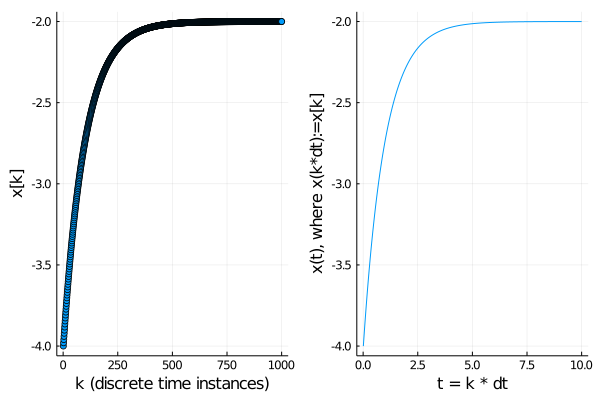
\includegraphics[width=0.6\textwidth]{graphicsAppendices/DiscreteTimeModel03.png}
\caption[]{Plot of the function $x:[0,10]\to \real$ that solves \eqref{eq:DiscreteEquation02} when its initial condition is $x[1]=4$. The discrete interval of time $\delta t = 0.01$ is small enough that it looks continuous, and in fact, if one connects the dots, our function versus time looks like a continuous curve.}
\label{fig:Proj03Plot03}
\end{figure}

\section{Equations with Derivatives in them are called Differential Equations}
\label{sec:ODEs4Real}
All of us hear about ``$F=ma$'' in High School, one of Newton's laws for how a body of mass $m$ accelerates under the action of applied forces $F$. We might also learn that ``acceleration'', $a$, is the rate of change of ``velocity'', $v$, with respect to time, $t$. 

\vspace*{0.5cm}
\begin{tcolorbox}[sharp corners, colback=green!30, colframe=green!80!blue, title=\textbf{\large The notation $\mathbf{\frac{d}{dt}}$}]
In Calculus, the rate of change of one quantity, say $v$, with respect to another quantity, say $t$, is denoted 
$$ \frac{dv(t)}{dt}.$$
Hence, in the language of Calculus, acceleration is related to velocity by
$$a(t) := \frac{dv(t)}{dt}, $$
which, once again, is just shorthand for ``acceleration is the rate of change of velocity with respect to time''. This course does not assume knowledge of Calculus, so please don't sweat the introduction of this notation. For us, it is just a shorthand way of saying ``rate of change with respect to time''.
\end{tcolorbox}

Using this shorthand notation, we can express Newton's Law as
\begin{equation}
    m \frac{dv(t)}{dt} =  F(t).  %\frac{1}{m}
\end{equation}
If we suppose that the body is falling in air, we might model the total force $F(t)$ acting on the body as being due to gravity and air friction, 
$$F(t) =  -mg -k_d v(t). $$
Doing so leads us to the equation
\begin{equation}
\label{eq:maEqualsDrag}
    \boxed{m\frac{dv(t)}{dt} = - k_d v(t) -g }.
\end{equation}
This equation says that the rate of change of the velocity as a function of time is given by a sum of two terms, one of which corresponds to gravity and the other to air resistance.
Equation~\eqref{eq:maEqualsDrag} is called a \textbf{differential equation}, that is, an equation that depends on ``derivatives.''\\

In \eqref{eq:maEqualsDrag}, let's now replace the shorthand Calculus symbol for rate of change, $\frac{dv(t)}{dt}$, with the same kind of numerical approximation we used in our studies of root finding and optimization, namely
\begin{equation}
\label{eq:dvdtFiniteDifference}
\frac{dv(t)}{dt} \approx \frac{v(t+\delta t)-v(t)}{\delta t}.
\end{equation}

Substituting \eqref{eq:dvdtFiniteDifference} into \eqref{eq:maEqualsDrag} and assuming the approximation is ``good enough'' (that we can change $\approx$ into $=$) give
\begin{equation}
\label{eq:maEqualsDragDiffrenceEq}
\begin{aligned}
\frac{dv(t)}{dt}  &= \frac{1}{m} \left( - k_d v(t) -g \right) \\
& \Updownarrow \\
    \frac{v(t+\delta t)-v(t)}{\delta t}& = \frac{1}{m} \left(- k_d v(t) -g \right) \\
    & \Updownarrow \\
  v(t+\delta t)-v(t) & = \delta t \frac{1}{m} \left(- k_d v(t) -g \right)\\
   & \Updownarrow \\
  v(t+\delta t) & = v(t) + \delta t \frac{1}{m} \left(- k_d v(t) -g \right).
  \end{aligned}
\end{equation}


If we then define $t = k \cdot \delta t$ and $v[k]:=v(k \cdot \delta t)$, the equation looks just like our \textit{difference equations} in Sec.~\ref{sec:DiscreteTime02}. Indeed, we have $v(t+\delta t) = v(k \cdot \delta t +\delta t) =  v((k+1)\cdot \delta t)=v[k+1]$, and \eqref{eq:maEqualsDragDiffrenceEq} becomes
\begin{equation}
\label{eq:maEqualsDragDiffrenceEq02}
v[k+1]  = v[k] - \delta t \frac{k_d}{m} v[k] - \delta t \frac{g}{m},
\end{equation}
which is very much like \eqref{eq:DiscreteEquation02} and hence, we now know one way to (approximately) solve the differential equation \eqref{eq:maEqualsDrag}: we set an initial condition and iterate based on \eqref{eq:maEqualsDragDiffrenceEq02}. \\

In fact, if the mass of our falling body is $m=\frac{2}{g}$ and its drag is $k_d=m$, then \eqref{eq:maEqualsDragDiffrenceEq02} is exactly the same as \eqref{eq:DiscreteEquation02}. Moreover, we can physically interpret the solution of the differential equation \eqref{eq:maEqualsDrag}, which is plotted in Fig.~\ref{fig:Proj03Plot03}, as a package is tossed out of plane. Our model tracks its evolution from the moment the parachute deploys, greatly increasing its drag, thereby slowing its velocity from an initial value of $-4$ to $-2$ units of distance per second (we never specified the units).

\section{Discretization of ODEs of Higher Dimension}

\vspace*{0.5cm}
\begin{tcolorbox}[sharp corners, colback=green!30, colframe=green!80!blue, title=\textbf{\large ODE}]
ODE is short for Ordinary Differential Equation. The word ``ordinary'' is used because there are other kinds of differential equations, which apparently, are less ``ordinary''. Everyone in the know uses the terminology ODE, hence you will too!
\end{tcolorbox}


ODEs can be vector valued too. A linear ODE may look like this,
$$\frac{dx(t)}{dt} = Ax(t) + b. $$
Just as before, we select $\delta t>0$ and define $x[k]:=x(k \cdot \delta t)$, and re-write the differential equation as a difference equation
\begin{align*}
    \frac{dx(t)}{dt} &\approx \frac{x(t+\delta t) - x(t)}{\delta t} \\
    &\Downarrow \\
 \frac{x(t+\delta t) - x(t)}{\delta t} & \approx Ax(t) + b\\
    &\Downarrow \\
   x(t+\delta t) &= x(t) + \delta t \left( Ax(t) + b \right)\\
   &\Downarrow \\
   x[k+1] & = x[k] + \delta t A x[k] + \delta t b
\end{align*}

A two-dimensional example is
\begin{equation}
    \label{eq:DiscreteEquation03}
    \underbrace{\left[\begin{array}{c}
x_1[k+1] \\ x_2[k+1]  \end{array}\right]}_{x[k+1]}=\underbrace{\left[\begin{array}{c}
x_1[k] \\ x_2[k]  \end{array}\right]}_{x[k]} + ~ \delta t \cdot \underbrace{\left[\begin{array}{rr}
0.0 & 1.0 \\
-2.0 & -1.0
 \end{array}\right]}_{A} \underbrace{\left[\begin{array}{c}
x_1[k] \\ x_2[k]  \end{array}\right]}_{x[k]}  +  ~\delta t \cdot \includecomment{}\underbrace{\left[\begin{array}{r}
0.0  \\1.0  \end{array}\right]}_{b}.
\end{equation}
This time, our $x[1]$ is a $2 \times 1$ vector. We'll arbitrarily specify it as $x[1]=[2~~0]^\top$. The plots of $x$ as a function of index $k$ and of time $t=k\cdot \delta t$ are given in Fig.~\ref{fig:Proj03Plot04}. The associated Julia code is given in Sec.~\ref{sec:CodeFigs04}.\\


Finally, not only can the function $x$ of time can be vector valued, it can have nonlinear terms. Here is a common example from physics: a pendulum of mass $m$ and length $\ell$ swinging from a frictionless pivot satisfies the equation
\begin{equation}
\label{eq:PendulumODE01}
\begin{aligned}
    \frac{d x_1(t)}{dt}&= x_2(t) \\
    \frac{d x_2(t)}{dt}&= -\frac{g}{\ell} \sin(x_1(t)),
\end{aligned}
\end{equation}
where $x_1$ is the angle of the pendulum and $x_2$ is its angular velocity. 
We'll rewrite the model in vector form by defining
\begin{equation}
    \label{eq:Statex}
    x := \left[\begin{array}{c}
        x_1 \\
         x_2
    \end{array} \right],
\end{equation}
so that
\begin{equation}
    \label{eq:Statex02}
    \frac{dx(t)}{dt} = \left[\begin{array}{c}
        \frac{dx_1(t)}{dt}  \\
         \frac{dx_2(t)}{dt} 
    \end{array} \right]:=  \underbrace{\left[\begin{array}{c}
        x_2(t) \\
          -\frac{g}{\ell} \sin(x_1(t))
    \end{array} \right]}_{f(x(t))} =: f(x(t))
\end{equation}

To find a solution, we discretize the model with $\delta t>0$. To show the flexibility we have in approximating the derivative, we'll use a symmetric difference approximation this time, namely
\begin{equation}
\label{eq:PendulumIntegration}
\begin{aligned}
    \frac{dx(t)}{dt} &\approx \frac{x(t+\delta t) - x(t- \delta t)}{ 2\delta t} \hspace*{.3cm}\text{and} \hspace*{.3cm}\frac{dx(t)}{dt} = f(x(t))\\
    &\Updownarrow \\
   x(t+\delta t) &= x(t-\delta t) + 2 \delta t f(x(t)) \hspace*{.3cm}\text{and} \hspace*{.3cm} t=k\cdot \delta t\\
   &\Updownarrow \\
   x[k+1] & = x[k-1] + \delta t f(x[k])
\end{aligned}
\end{equation}
We use the last line of \eqref{eq:PendulumIntegration} to iterate and compute a solution to the pendulum ODE \eqref{eq:PendulumODE01}. The solution is plotted in Fig.~\ref{fig:Proj03Plot05}. The associated Julia code is given in Sec.~\ref{sec:CodeFigs05}.  

\begin{tcolorbox}
Our transformation of ODEs into difference equations are examples of numerical integration methods. When we use the approximation 
$$\frac{dx(t)}{dt} \approx \frac{x(t + \delta t)-x(t)}{\delta t }  $$
we end up with what is called a first-order forward Euler integration method. In general, it's a pretty bad way to solve ODEs, but for a first introduction, it is great! We can do a lot with it.
\end{tcolorbox}

% \begin{equation}
%     \label{eq:DiscreteEquation04}
%     \underbrace{\left[\begin{array}{c}
% x_1[k+1] \\ x_2[k+1]  \end{array}\right]}_{x[k+1]}=\underbrace{\left[\begin{array}{c}
% x_1[k-1] \\ x_2[k-1]  \end{array}\right]}_{x[k-1]} +   ~\delta t \cdot \includecomment{}\underbrace{\left[\begin{array}{c}
% x_2[k] \\-\frac{g}{\ell} \sin(x_1[k]) \end{array}\right]}_{f(x[k])},
% \end{equation}

\begin{figure}[t!]
\centering
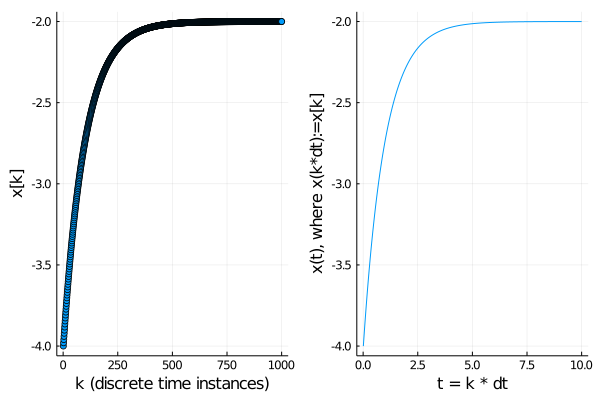
\includegraphics[width=0.6\textwidth]{graphicsAppendices/DiscreteTimeModel03.png}
\caption[]{Plot of the function $x:[0,10]\to \real$ that solves \eqref{eq:DiscreteEquation02} when its initial condition is $x[1]=4$. The discrete interval of time $\delta t = 0.01$ is small enough that it looks continuous, and in fact, if one connects the dots, our function versus time looks like a continuous curve.}
\label{fig:Proj03Plot03B}
\end{figure}

%\newpage


\begin{figure}[hbt!]
\centering
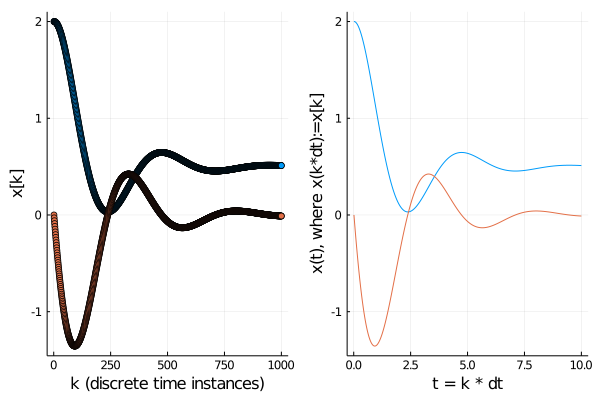
\includegraphics[width=0.7\textwidth]{graphicsAppendices/DiscreteTimeModel04.png}
\caption[]{Plot of the vector valued function $x:[0,10]\to \real^2$ solving the ODE $\frac{dx(t)}{dt }= Ax +b$, with the solution approximated in  \eqref{eq:DiscreteEquation03}. The discrete interval of time is small enough that it looks continuous!}
\label{fig:Proj03Plot04}
\end{figure}

\begin{figure}[hbt!]
\centering
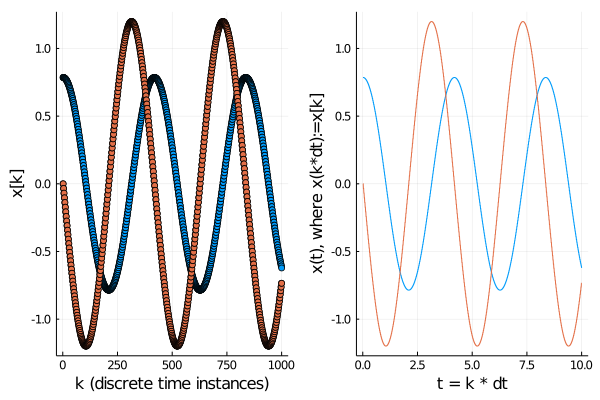
\includegraphics[width=0.7\textwidth]{graphicsAppendices/DiscreteTimeModel05.png}
\caption[]{Plot of a vector valued function $x:[0,10]\to \real^2$  that oscillates back and forth because it corresponds to the solution the pendulum ODE given in \eqref{eq:PendulumODE01}. The blue lines are the angle of the pendulum and the brown(ish) lines are its angular velocity.}
\label{fig:Proj03Plot05}
\end{figure}

\clearpage


\section{Julia Code for Generating the Figures}

We provide code in Julia 1.41 for the figures appearing in this Appendix.

\subsection{For Figures~\ref{fig:Proj03Plot01} and ~\ref{fig:Proj03Plot02}}
\label{sec:CodeFigs0102}

\begin{lstlisting}[language=Julia]

# Model 
dt=0.01
T=10
N=floor(Int,T/dt);
K=1:N
time = K*dt
x=zeros(N,1)
x[1]=-4
for k=1:(N-1)
    x[k+1]=(1-dt)*x[k]-2*dt
end
# Plotting 
plot1=scatter(K,x,xlabel="k (discrete time instances)", ylabel="x[k]", leg=false)
plot2=plot(time,x,xlabel="t = k * dt", ylabel="x(t), where x(k*dt):=x[k]", leg=false)
plot(plot1, plot2, layout = (1, 2), legend = false)
#Turn the plot into an image that one can copy
plot!(fmt = :png) 

\end{lstlisting}

\subsection{Code for Figure~\ref{fig:Proj03Plot03}}
\label{sec:CodeFigs03}

\begin{lstlisting}[language=Julia]
using Plots
gr()
# Model 
N=20
time=1:N
x=zeros(N,1)
x[1]=4
for k=1:(N-1)
    x[k+1]=0.5*x[k]+1
end
# Plotting
scatter(time,x)
#plot!(xlabel="k (discrete time instances)", ylabel="x[k]", 
#title="Plot of as a function of time: Discrete-time Model", leg=false)
plot!(xlabel="k (discrete time instances)", ylabel="x[k]", leg=false)
#Turn the plot into an image that one can copy
plot!(fmt = :png)
#
# Second plot
#
plot(time,x)
#plot!(xlabel="k (discrete time instances)", ylabel="x[k]", 
#title="Plot of as a function of time: Discrete-time Model", leg=false)
plot!(xlabel="k (discrete time instances)", ylabel="x[k]", leg=false)
scatter!(time,x)
#Turn the plot into an image that one can copy
plot!(fmt = :png)  
\end{lstlisting}

\subsection{Code for Figure~\ref{fig:Proj03Plot03B}}
\label{sec:CodeFigs03B}
\begin{lstlisting}[language=Julia]
# Model 
dt=0.01
T=10
N=floor(Int,T/dt);
K=1:N
time = K*dt
x=zeros(N,1)
x[1]=4
for k=1:(N-1)
    x[k+1]=(1-dt)*x[k]+2*dt
end
# Plotting 
plot1=scatter(K,x,xlabel="k (discrete time instances)", ylabel="x[k]", leg=false)
plot2=plot(time,x,xlabel="t = k * dt", ylabel="x(t), where x(k*dt):=x[k]", leg=false)
plot(plot1, plot2, layout = (1, 2), legend = false)
#Turn the plot into an image that one can copy
plot!(fmt = :png)  
\end{lstlisting}

\subsection{Code for Figure~\ref{fig:Proj03Plot04}}
\label{sec:CodeFigs04}



\begin{lstlisting}[language=Julia]
# Model 
dt=0.01
T=10
N=floor(Int,T/dt);
K=1:N
time = K*dt
A=[0 1; -2 -1]
b=[0;1]
x=zeros(N,2)
x[1, :]=[2 0]
for k=1:(N-1)
    x[k+1,:]=x[k,:]+ dt*A*x[k,:] + dt*b
end
# Plotting 
plot1=scatter(K,x,xlabel="k (discrete time instances)", ylabel="x[k]", leg=false)
plot2=plot(time,x,xlabel="t = k * dt", ylabel="x(t), where x(k*dt):=x[k]", leg=false)
plot(plot1, plot2, layout = (1, 2), legend = false)
#Turn the plot into an image that one can copy
plot!(fmt = :png) 
\end{lstlisting}

\subsection{Code for Figure~\ref{fig:Proj03Plot05}}
\label{sec:CodeFigs05}

\begin{lstlisting}[language=Julia]
# Model 
dt=.01
T=50
N=floor(Int,T/dt);
K=1:N
time = K*dt
g=9.81 #m/s^2
l=4 # m
x=zeros(N,2)
#Pendulum equations
f(x1,x2)=[x2;-(g/l)*sin(x1)]
#Initial conditions
x[1, :]=[pi/4 0]
x[2, :]=x[1,:] + dt*f(x[1,1],x[1,2])
#Euler integration based on Symmetric Difference for dx/dt
for k=2:(N-1)
x[k+1,:]=x[k-1,:] +2*dt*f(x[k,1],x[k,2])
end
# Plotting 
plot1=scatter(K,x,xlabel="k (discrete time instances)", ylabel="x[k]", leg=false)
plot2=plot(time,x,xlabel="t = k * dt", ylabel="x(t), where x(k*dt):=x[k]", leg=false)
plot(plot1, plot2, layout = (1, 2), legend = false)
#Turn the plot into an image that one can copy
plot!(fmt = :png) 
\end{lstlisting}


